% Independently reviewed exact families restored from July 2026 material.
% All parameters satisfy strict contraction; a=0 and r=0 are excluded.
\section{Exact families across the three orientation types}
\label{sec:restored-exact-families}

For $0<t<1$, define the signed digit set
\begin{equation}\label{eq:restored-Ct}
 C_t=\left\{\sum_{n=0}^{\infty}e_nt^n:
               e_n\in\{-1,1\}\right\}.
\end{equation}
It is a Cantor set when $t<1/2$ and equals
\[
 I_t=\left[-\frac1{1-t},\frac1{1-t}\right]
\]
when $t\ge1/2$. Indeed, the intervals $-1+tI_t$ and $1+tI_t$
are disjoint for $t<1/2$ and cover $I_t$ for $t\ge1/2$.
In the first case the two maps satisfy strong separation, and
$\dim_H C_t=\log2/(-\log t)$.

\subsection{Two complete opposite--opposite families}

For $0<|a|<1$ compare the two systems
\begin{align}
 f_e(z)&=e+a\overline z,
             &&e\in\{-1,1\},\label{eq:restored-OO-diagonal}\\
 \widetilde f_e(z)&=e+ea\overline z,
             &&e\in\{-1,1\}.\label{eq:restored-OO-antidiagonal}
\end{align}
Their normalized coefficient pairs are respectively $(a,a)$ and
$(-a,a)$.

\begin{theorem}[Exact opposite--opposite phase diagram]
\label{thm:restored-OO}
Both systems have the same attractor and the same labelled geometric
first-level pieces. With $t=|a|^2$,
\begin{equation}\label{eq:restored-OO-set}
 K_a=C_t+aC_t,\qquad
 K_{a,-}=-1+tC_t+aC_t,\quad
 K_{a,+}=1+tC_t+aC_t.
\end{equation}
Their coding maps are related by a first-symbol-preserving
homeomorphism of the binary address space.

If $a\notin\mathbb R$, the following alternatives are exact.
\begin{enumerate}
\item For $|a|<2^{-1/2}$, the attractor is a real-linear image of
      $C_t\times C_t$, its two pieces are disjoint, and
      $\dim_H K_a=\log2/(-\log|a|)$.
\item For $|a|=2^{-1/2}$, the attractor is the parallelogram
      $I_t+aI_t$ and its contact set is the segment $aI_t$.
\item For $|a|>2^{-1/2}$, the attractor is the parallelogram
      $I_t+aI_t$ and its contact is the positive-area parallelogram
      \begin{equation}\label{eq:restored-OO-Q}
      Q_a=J_t+aI_t,\qquad
      J_t=\left[-\frac{2t-1}{1-t},\frac{2t-1}{1-t}\right].
      \end{equation}
\end{enumerate}
For $t\ge1/2$ their areas are
\begin{equation}\label{eq:restored-OO-areas}
 m_2(K_a)=\frac{4|\operatorname{Im}a|}{(1-t)^2},\qquad
 m_2(Q_a)=\frac{4(2t-1)|\operatorname{Im}a|}{(1-t)^2}.
\end{equation}
For real $a$, put $r=|a|$. Then $K_a=C_r$ and
\[
 Q_a=\varnothing\quad(0<r<1/2),\qquad
 Q_a=\left[-\frac{2r-1}{1-r},\frac{2r-1}{1-r}\right]
           \quad(1/2\le r<1).
\]
Thus the real transition is from a Cantor set to an interval with
point contact at $r=1/2$, and then to an interval with interval contact.
\end{theorem}

\begin{proof}
The real-linear map $A(z)=a\overline z$ satisfies $A^2=t\,\mathrm{id}$.
For the diagonal system, the coding series therefore splits as
\begin{equation}\label{eq:restored-OO-coding}
 \pi_{\mathrm{diag}}(e)
 =\sum_{k\ge0}e_{2k}t^k+a\sum_{k\ge0}e_{2k+1}t^k.
\end{equation}
The even and odd signs vary independently, proving the formula for
$K_a$. Applying either generator and using $C_t=-C_t$ gives the two
piece formulas in \eqref{eq:restored-OO-set}.

For the anti-diagonal system, its length-$n$ linear part is the
product of the first $n$ signs times $A^n$. Consequently
\[
 \pi_{\mathrm{anti}}(e)=\pi_{\mathrm{diag}}(\Phi(e)),\qquad
 \Phi(e)_n=\prod_{j=0}^n e_j.
\]
This map preserves the first symbol and is a homeomorphism: its
inverse is $e_0=d_0$ and $e_n=d_{n-1}d_n$ for $n\ge1$.
It identifies the labelled first pieces as well as the full
attractors. No commutation with the shift is asserted.

When $a$ is nonreal, $(x,y)\mapsto x+ay$ is an invertible real-linear
map. The product representation gives all asserted set types.
For $t<1/2$ the two intervals containing $-1+tC_t$ and $1+tC_t$
are separated, and linear independence of $1,a$ makes the two
planar pieces disjoint. The product has four strongly separated
similarities of ratio $t$, so its Hausdorff dimension is
$\log4/(-\log t)=\log2/(-\log|a|)$.
For $t\ge1/2$, intersecting the coordinate rectangles gives
$J_t\times I_t$. The absolute determinant of the real-linear map
is $|\operatorname{Im}a|$, giving \eqref{eq:restored-OO-areas}.

When $a$ is real, the even and odd series interleave into $C_r$;
the signs of $a$ can be absorbed into independent digit signs.
The common first pieces are $-1+rC_r$ and $1+rC_r$.
Their interval intersection gives the stated formula for $Q_a$.
\end{proof}

\begin{corollary}[Exact discontinuous radial frontier]
\label{cor:restored-OO-frontier}
Let $\mathcal M_{OO}$ be the connectedness locus in the full
four-real-dimensional opposite--opposite parameter domain. For
either embedding $\iota(a)=(a,a)$ or $\iota(a)=(-a,a)$,
\begin{align}
 \iota^{-1}(\mathcal M_{OO})
   &=\{a:2^{-1/2}\le|a|<1\}
     \cup\{a\in\mathbb R:1/2\le|a|<1\},
       \label{eq:restored-OO-connectedness}\\
 \iota^{-1}(\partial\mathcal M_{OO})
   &=\{a:|a|=2^{-1/2}\}
     \cup\{a\in\mathbb R:1/2\le|a|\le2^{-1/2}\}.
       \label{eq:restored-OO-fullboundary}
\end{align}
Writing $a=\rho^{-1}e^{i\theta}$, the connected values on a fixed ray
are exactly $1<\rho\le R(\theta)$, where
\begin{equation}\label{eq:restored-OO-radial}
 R(\theta)=
 \begin{cases}
 2,&\theta\equiv0\pmod\pi,\\
 \sqrt2,&\theta\not\equiv0\pmod\pi.
 \end{cases}
\end{equation}
\end{corollary}

\begin{proof}
The connectedness formula is the theorem. Every nonreal point of
$|a|=2^{-1/2}$ is approached along the same ray by disconnected
systems with smaller modulus. The real points on the stated
segments are approached by nonreal parameters of modulus less than
$2^{-1/2}$, also disconnected. The same construction works at the
two real endpoints of the circle. All these connected systems are
therefore boundary points of the full parameter locus.
Conversely, when $|a|>2^{-1/2}$ the strict inequality
$|a|^2+|a|^2>1$ places the parameter in the full connectedness
interior. All remaining slice parameters are disconnected, and
the disconnectedness set is open. This proves the full-boundary
formula, not just a statement about boundary relative to the slice.
Substitution of $\rho=1/|a|$ gives \eqref{eq:restored-OO-radial}.
\end{proof}

The jump is caused by the rank loss of $(x,y)\mapsto x+ay$ on the
real axis. It gives an exact example in which a radial frontier
function is discontinuous. A continuous interpolated shell can
therefore omit connected boundary segments, even on a slice whose
radial membership is completely understood.

\begin{figure}[tbp]
\centering
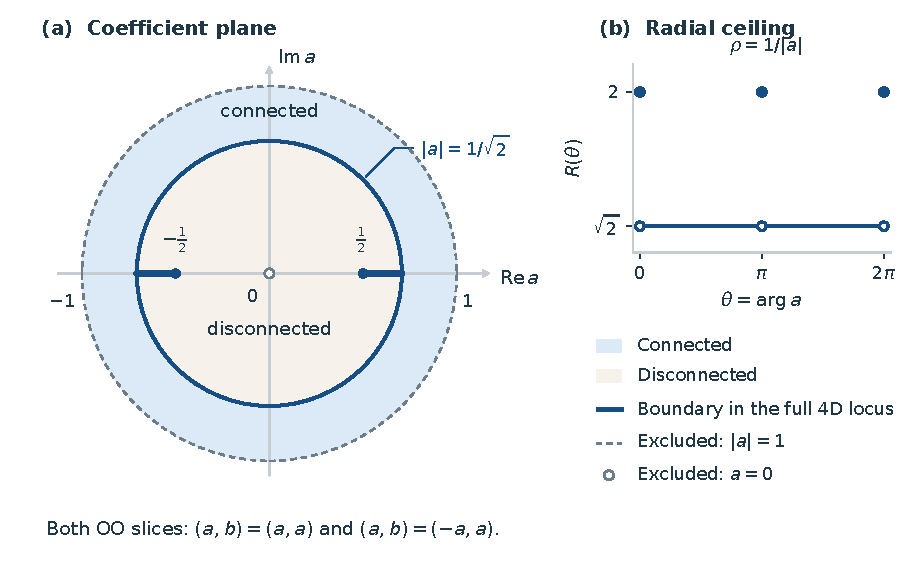
\includegraphics[width=.94\linewidth]{figures/oo_phase_diagram.pdf}
\caption{Exact opposite--opposite coefficient slices. The connected region and
its intersection with the full four-dimensional boundary follow from
Corollary~\ref{cor:restored-OO-frontier}. The real antennae produce the jumps in
the radial ceiling. The unit circle is outside the strict contraction domain.}
\label{fig:oo-phase}
\end{figure}

\subsection{A common quarter-turn family in all orientation types}

For $0<r<1$ consider the following four marked systems:
\begin{align*}
 \mathrm{DD}:&\quad f_e(z)=e+irz,\\
 \mathrm{DO}:&\quad f_-(z)=-1+irz,\qquad
                    f_+(z)=1+ir\overline z,\\
 \mathrm{OO}:&\quad f_e(z)=e+ir\overline z,\\
 \widetilde{\mathrm{OO}}:&\quad
                    f_e(z)=e+eir\overline z.
\end{align*}

\begin{theorem}[Quarter-turn equivalence across orientation types]
\label{thm:restored-quarter-turn}
All four systems have the same attractor $K_r$, the same labelled
first-level pieces, and the same geometric contact set. With
$t=r^2$,
\begin{equation}\label{eq:restored-quarter-set}
 K_r=C_t+irC_t,\qquad
 K_{r,\pm}=\pm1+tC_t+irC_t.
\end{equation}
Their coding maps are related by explicit first-symbol-preserving
homeomorphisms of the address space.

For $r<2^{-1/2}$, the attractor is a Cantor product with
$\dim_HK_r=\log2/(-\log r)$ and empty first-piece contact. At
$r=2^{-1/2}$,
\begin{equation}\label{eq:restored-quarter-critical}
 K_r=[-2,2]+i[-\sqrt2,\sqrt2],\qquad
 Q_r=i[-\sqrt2,\sqrt2].
\end{equation}
For $r>2^{-1/2}$, the attractor and its contact are the rectangles
\[
 K_r=I_t+irI_t,\qquad Q_r=J_t+irI_t.
\]
In particular, the critical parameter lies on the boundary of the
full connectedness locus in each of the three orientation types.
\end{theorem}

\begin{proof}
The two OO cases follow from Theorem~\ref{thm:restored-OO} with $a=ir$.
Use the diagonal OO coding map as the reference. In the DD case,
splitting even and odd powers of $ir$ gives
\[
 \pi_{DD}(e)=\sum_{k\ge0}(-1)^ke_{2k}t^k
              +ir\sum_{k\ge0}(-1)^ke_{2k+1}t^k.
\]
Thus $\pi_{DD}=\pi_{OO}\circ\Phi_{DD}$, where
\[
 \Phi_{DD}(e)_{2k}=(-1)^ke_{2k},\qquad
 \Phi_{DD}(e)_{2k+1}=(-1)^ke_{2k+1}.
\]
This coordinatewise involution preserves $e_0$.

For the mixed system put
$E_k=\prod_{j=0}^ke_{2j}$ and
$O_k=\prod_{j=0}^ke_{2j+1}$. A composition of two consecutive
linear parts is multiplication by $e_{2j}t$ when acting on a real
digit. Grouping these pairs, and then treating the leading odd
factor, yields
\[
 \pi_{DO}(e)=\sum_{k\ge0}E_kt^k+ir\sum_{k\ge0}O_kt^k.
\]
Equivalently, the coefficient before the digit at position $2k$ is
$E_{k-1}t^k$, and the coefficient before the digit at position
$2k+1$ is $irO_{k-1}t^k$, with empty products equal to one.
These formulas also follow directly by induction on prefix length.
Therefore $\pi_{DO}=\pi_{OO}\circ\Phi_{DO}$ with
\[
 \Phi_{DO}(e)_{2k}=E_k,\qquad
 \Phi_{DO}(e)_{2k+1}=O_k.
\]
Its continuous inverse is given by
$e_0=E_0$, $e_1=O_0$ and
$e_{2k}=E_{k-1}E_k$, $e_{2k+1}=O_{k-1}O_k$ for $k\ge1$.
This map also preserves the first symbol.

First-symbol preservation transfers the two geometric pieces and
their intersection, as well as the attractor itself. The phase
classification follows from Theorem~\ref{thm:restored-OO}.
For every one of the four presentations, approaching the critical
value with $r<2^{-1/2}$ supplies a sequence of disconnected systems in
the same orientation type. The critical system is connected, so
it lies on the full parameter-space boundary.
\end{proof}

\begin{proposition}[Address multiplicity on the critical interface]
\label{prop:restored-interface-addresses}
In any of the four critical presentations, write a contact point
as $z=iry$, where $r=2^{-1/2}$ and $-2\le y\le2$. If
$u=(y+2)/4$ is an interior dyadic rational, $z$ has four addresses;
otherwise it has two addresses, including at $y=\pm2$.
The number of address pairs $(\omega,\eta)$ representing $z$ with
$\omega_0=-1$ and $\eta_0=1$ is respectively four or one.
\end{proposition}

\begin{proof}
In the reference OO coding, zero real coordinate for an address
beginning with $-1$ forces every subsequent even digit to be $1$:
$-1+\sum_{k\ge1}e_{2k}2^{-k}=0$ attains the maximum possible tail.
An address beginning with $1$ similarly forces all subsequent even
digits to be $-1$. On either side the free odd digits code
$y=\sum_{k\ge0}e_{2k+1}2^{-k}$. This is the usual binary coding of
$u=(y+2)/4$, which has two expansions exactly at the interior
dyadic rationals and one elsewhere. Thus each side supplies two
addresses or one address, respectively. Adding counts gives four
or two total addresses; multiplying the two side counts gives
four or one cross-piece pairs. The first-symbol-preserving
recodings transfer these counts to the other presentations.
\end{proof}

This interface has uncountably many geometric contact points, even
though all but countably many of them have exactly one address
from each first piece. Geometric contact cardinality and address
multiplicity are distinct data in an atlas of connected families.

\begin{figure}[tbp]
\centering
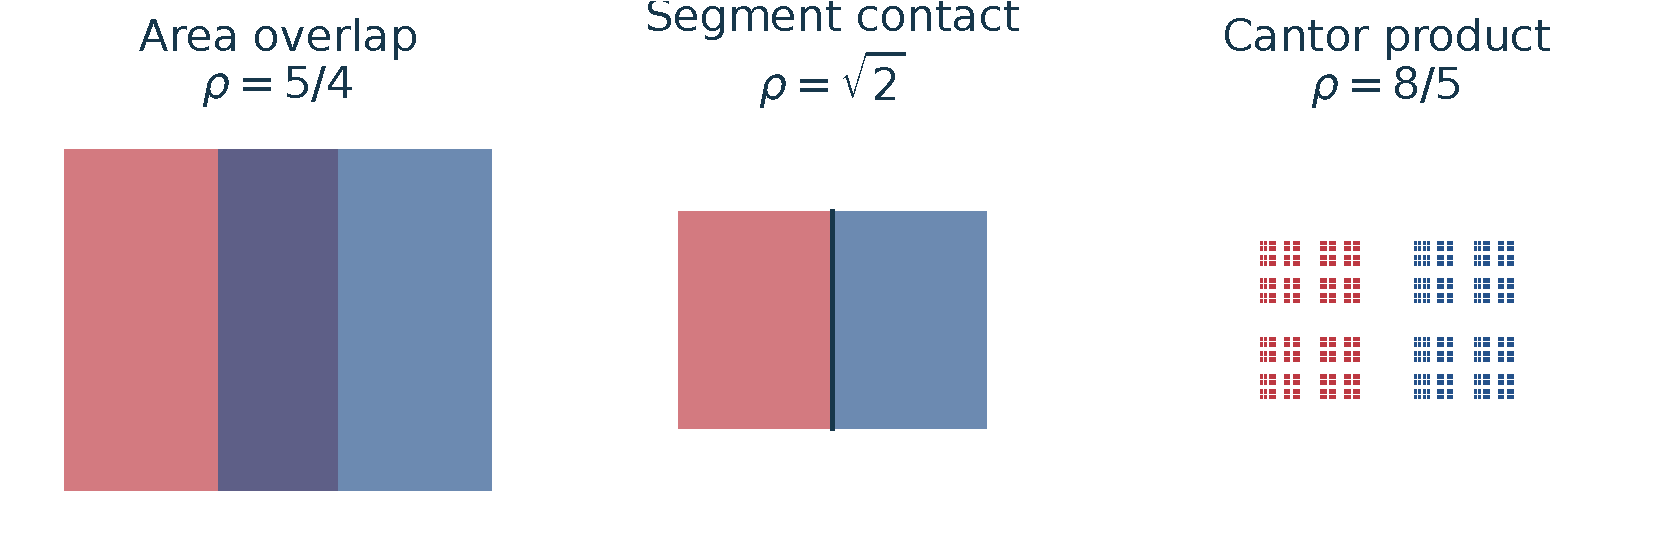
\includegraphics[width=\linewidth]{figures/quarter_turn_transition.pdf}
\caption{The common quarter-turn family of
Theorem~\ref{thm:restored-quarter-turn}, with $r=1/\rho$. Red and blue distinguish
the first-level pieces in each presentation. The first two panels are exact
rectangles and their contact. The last panel shows finite product-cylinder
covers of the Cantor attractor, using five terms in each real factor.
These are three parameter values from an exact phase classification.}
\label{fig:quarter-turn}
\end{figure}
